\documentclass[11pt]{article}
\usepackage[utf8]{inputenc}
\usepackage[T1]{fontenc}
\usepackage[margin=1in]{geometry}
\usepackage{amsmath}
\usepackage{booktabs}
\usepackage{graphicx}
\usepackage{float}
\usepackage{caption}
\usepackage{array}
\usepackage{tabularx}
\usepackage{orcidlink}
\usepackage{hyperref}
\usepackage[numbers]{natbib}
\hypersetup{colorlinks=true,allcolors=black}
\graphicspath{{figures/}}
\setlength{\textfloatsep}{7pt plus 2pt minus 2pt}
\setlength{\floatsep}{7pt plus 2pt minus 2pt}
\setlength{\intextsep}{7pt plus 2pt minus 2pt}
\captionsetup{skip=3pt}

\title{\textbf{Explaining Crop-Yield Anomalies with Multi-Method Interpretable Machine Learning}}
\author{
\begin{tabular}{c}
Tran Dai Phong Lam~\orcidlink{0009-0003-9320-8782}\thanks{Corresponding author.}, Thu Le~\orcidlink{0009-0008-3480-8311}\\
Nguyen Quoc Hung~\orcidlink{0009-0002-7538-7978}, Nguyen Trung Trinh~\orcidlink{0009-0003-5566-3469}\\[0.4em]
\small FPT University, Ho Chi Minh City, Vietnam\\
\small \href{mailto:phonglam2599@gmail.com}{\texttt{phonglam2599@gmail.com}},
\href{mailto:thulvn@fpt.edu.vn}{\texttt{thulvn@fpt.edu.vn}}\\
\small
\href{mailto:hungtvt2222@gmail.com}{\texttt{hungtvt2222@gmail.com}},
\href{mailto:trinhnguyen112355@gmail.com}{\texttt{trinhnguyen112355@gmail.com}}
\end{tabular}
}
\date{}

\begin{document}
\maketitle

\begin{abstract}
Yield prediction does not by itself explain why particular crop-state-years fall
below their long-run expectation. This study combines detrended low-yield anomaly
screening with a multi-method interpretable machine-learning protocol to identify
which extreme-weather driver groups are consistently emphasized by a fitted residual
model. We use a U.S. crop-state-year panel for Barley, Canola, Oats, and Wheat from
1990--2025, with USDA yield data and NASA POWER weather features. Linear detrending
within crop-state series flags 214 of 1,257 observations as low-yield anomalies using
$z<-1.0$. ExtraTrees yield models retain strong forward-time skill, while the
residual model is treated as a diagnostic explanation surface rather than a
high-skill anomaly-magnitude forecaster. We compare SHAP, grouped SHAP, group
permutation, group ablation, ALE curves, and selected LIME case studies. Heat is the
strongest global model-reliance signal, while anomaly-focused explanations show
co-leading heat and drought signals across methods. The contribution is a
reproducible rank-support protocol for cautious model-based explanation rather than
causal event attribution.
\end{abstract}

\noindent\textbf{Keywords:} crop yield; yield anomaly; explainable machine learning; SHAP; permutation importance; drought; heat stress.

\section{Introduction}
Crop-yield machine learning is often evaluated by average predictive accuracy, but
decision-makers also need to understand low-yield anomaly years. A model that
predicts yield levels well can still leave open a diagnostic question: which physical
weather drivers does the fitted model associate with below-trend crop outcomes? This
distinction matters because prediction and explanation can diverge, especially when
weather variables are correlated and yield anomalies are rare.

This paper reframes the task as multi-method model explanation. We first detrend
yield within crop-state series and flag unusually low residual years. We then train a
weather-yield residual model and compare explanation methods that operate at feature,
driver-group, and selected event levels. The central question is: which
extreme-weather driver groups are consistently emphasized by the fitted residual
model across several interpretable machine-learning methods?

The study makes three contributions. First, it combines crop-state yield detrending
with low-yield anomaly screening to separate long-run production trends from
short-run weather-sensitive deviations. Second, it implements a shared driver-group
XAI protocol that compares feature-level SHAP, grouped SHAP, group permutation, group
ablation, ALE response curves, and selected LIME explanations. Third, it evaluates
method agreement at global and anomaly-focused levels, allowing driver claims to be
stated more cautiously when several methods identify the same weather-driver group.

The analysis avoids causal overclaiming. Terms such as driver, attribution, and
explanation are used in a model-based diagnostic sense. Agreement across methods
means that the fitted model repeatedly identifies the same driver group; it does not
prove a real-world causal mechanism or formal climate-event attribution.

\begin{figure}[!htbp]
  \centering
  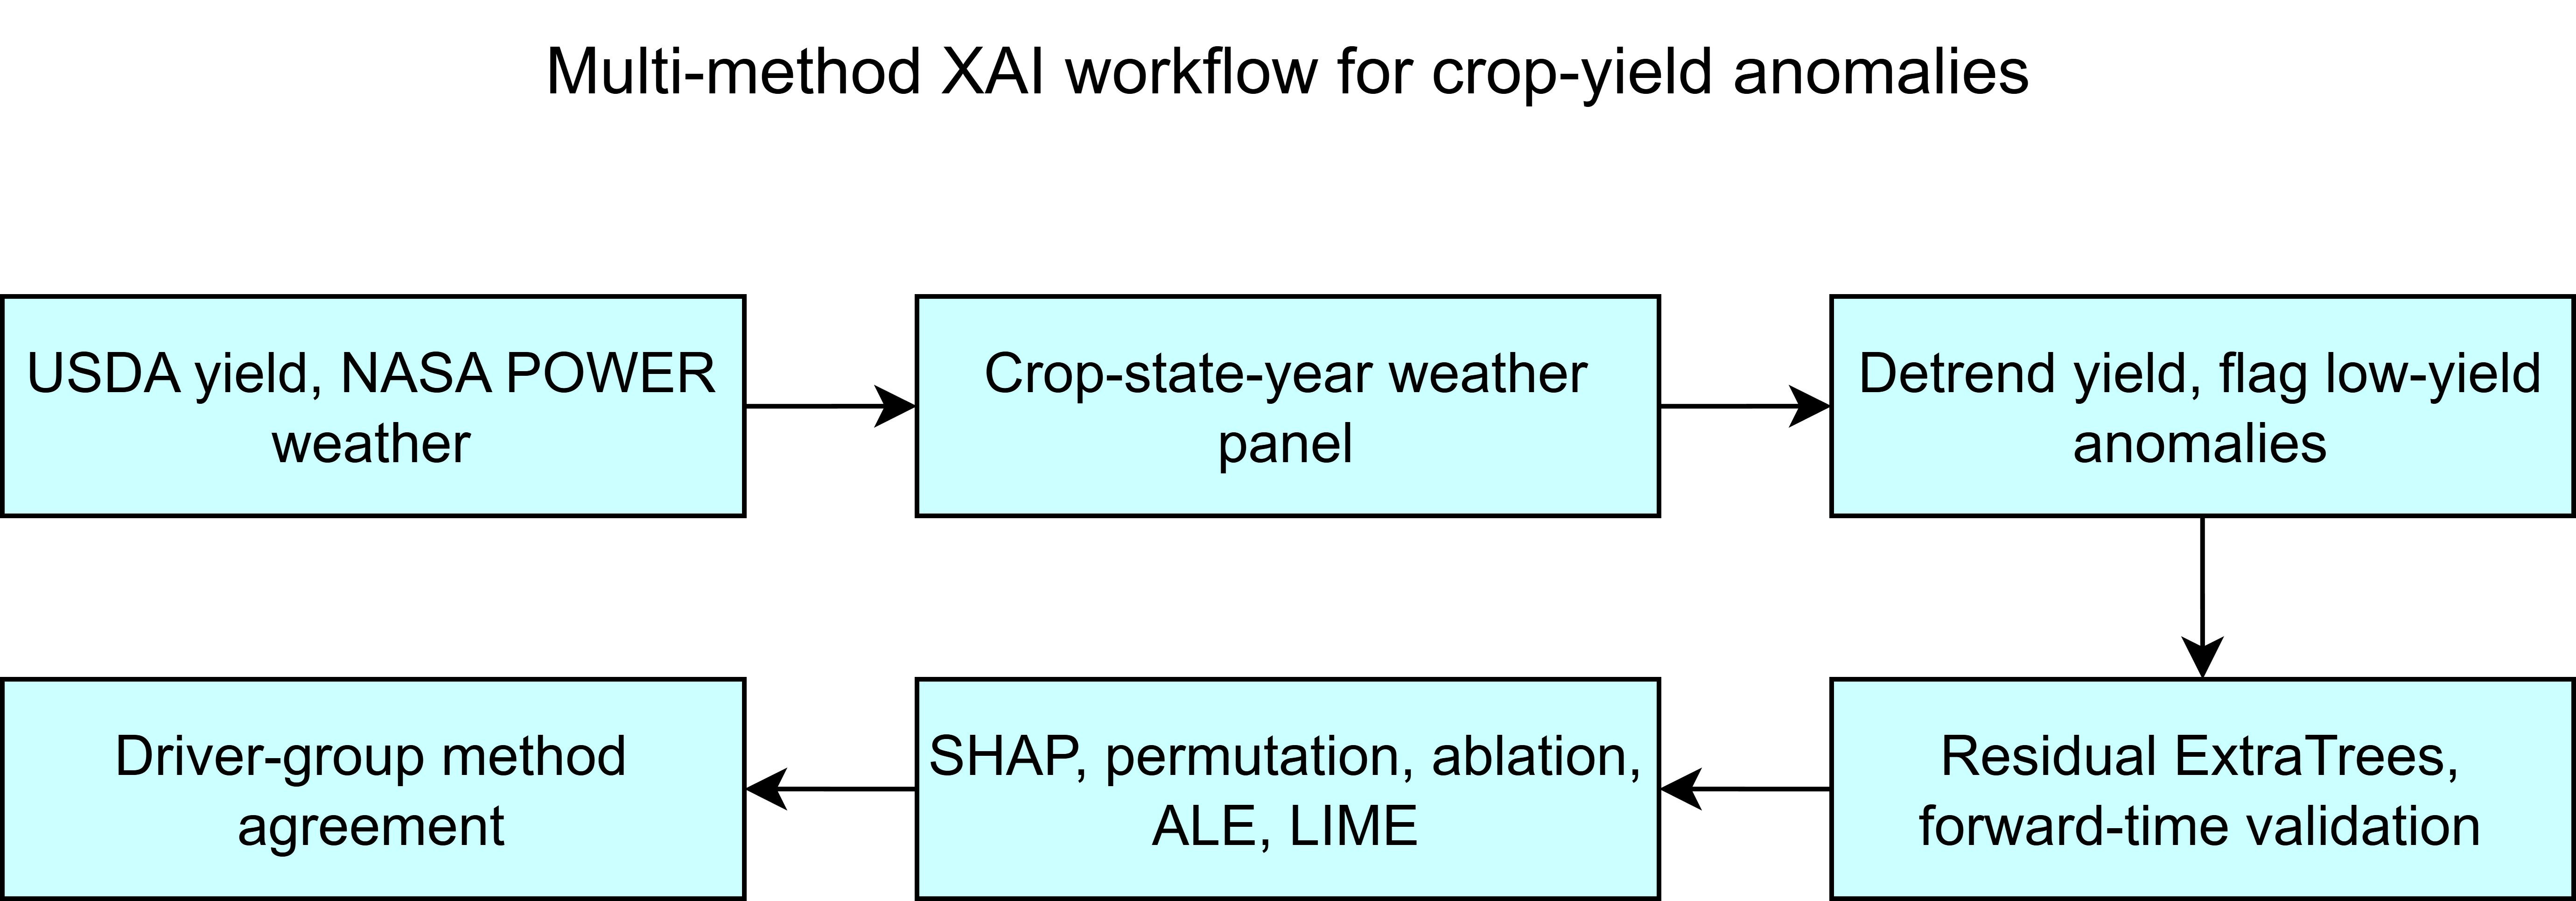
\includegraphics[width=0.95\linewidth]{fig01_method_workflow.png}
  \caption{Workflow for detecting detrended low-yield anomalies, fitting residual
  models, applying multiple explanation methods, and comparing driver-group support.}
  \label{fig:workflow}
\end{figure}

\section{Related Work}
Machine-learning yield studies show that weather and climate variables can support
crop prediction across regions and crops
\citep{Paudel2021,Meroni2021,Khaki2019,LengHall2020}. A related literature links
yield anomalies to weather extremes, including drought, heat, excess water, and cold
stress \citep{Lesk2016,Zampieri2017,Vogel2019,Heino2023,Schierhorn2021,Sjulgard2023}.
Because technological and management trends can dominate raw yield trajectories,
detrending is a standard step before interpreting weather-related yield variability
\citep{Ray2015,Lu2017,Meng2024}.

Explainable machine learning offers complementary tools for interpreting fitted
models. SHAP provides additive feature contributions \citep{LundbergLee2017}; LIME
offers selected local surrogate explanations \citep{Ribeiro2016}; model-reliance and
permutation ideas support grouped dependence checks \citep{Fisher2019}; and ALE
curves summarize response shape while reducing unrealistic feature combinations that
can affect simple partial-dependence displays \citep{ApleyZhu2020}. Rather than
treating any single method as decisive, this study compares whether several methods
point to the same physically meaningful driver groups.

\section{Data}
The unit of analysis is a crop-state-year. The processed frame contains 1,257
observations from 1990--2025 for Barley, Canola, Oats, and Wheat across 12 U.S.
states: Colorado, Illinois, Iowa, Kansas, Minnesota, Montana, Nebraska, North Dakota,
Oklahoma, South Dakota, Texas, and Washington. Yield is measured in t ha$^{-1}$ from
USDA NASS \citep{USDANASSQuickStats}. Weather features are derived from NASA POWER
daily data \citep{NASAPOWER2025} and summarized over crop growing-season windows
labelled spring or winter.

Each row contains crop identity, state identity, year, growing-season window, yield,
representative state latitude and longitude, and aggregated weather indicators. The
weather extraction uses representative state coordinates rather than gridded or
crop-area-weighted weather. Therefore, explanations should be interpreted at a
state-representative scale; within-state heterogeneity in soils, irrigation, cultivar,
and management is not resolved. The panel is moderately unbalanced: Canola has fewer
observations and fewer states than Oats or Wheat, so crop-specific patterns should
not be generalized equally across crops.

The XAI analysis uses 35 full-season weather features grouped into heat, drought,
frost/cold, excess rain, and radiation. Numerical predictors are median-imputed and
standardized inside the model pipeline; crop and state identifiers are imputed by
most frequent category and one-hot encoded. The same preprocessing pipeline is used
for yield and residual models. The feature set includes rainfall totals, wet days,
dry spells, heat days, heatwave summaries, frost days, and radiation summaries.

\input{tables/table01_dataset_summary.tex}
\begin{table}[!htbp]
\centering
\caption{Extreme-weather driver groups used in the multi-method XAI analysis.}
\label{tab:driver_groups}
\resizebox{\linewidth}{!}{%
\begin{tabular}{@{}lll@{}}
\toprule
driver\_group & description & n\_features \\
\midrule
heat & High temperature, heatwave, and growing-degree exposure & 12 \\
drought & Low rainfall, dry spells, and hot-dry compound stress & 8 \\
frost\_cold & Cold nights, frost days, and low minimum-temperature stress & 5 \\
excess\_rain & Heavy rainfall, wetness, and short-duration rainfall maxima & 8 \\
radiation & Seasonal solar-radiation anomalies & 2 \\
\bottomrule
\end{tabular}
}
\end{table}


\section{Method}
\subsection{Anomaly Screening}
For each crop-state series, yield $y_{c,s,t}$ is linearly detrended against year:
\begin{equation}
  y_{c,s,t} = \alpha_{c,s} + \beta_{c,s}t + e_{c,s,t}.
\end{equation}
The residual is standardized within the crop-state series,
\begin{equation}
  z_{c,s,t} = \frac{e_{c,s,t}}{\operatorname{sd}(e_{c,s,\cdot})},
\end{equation}
using sample standard deviation. An observation is flagged as a low-yield anomaly
when $z<-1.0$. Robustness checks use stricter thresholds of $z<-1.5$ and $z<-2.0$,
and compare the linear-trend anomaly set with a centered seven-year rolling-trend
baseline.

\subsection{Yield and Residual Models}
The yield baseline uses ExtraTrees with year, location, crop, state, and weather
features \citep{Geurts2006,Pedregosa2011}. Its role is to check whether the data
contain substantial predictive signal for yield levels. The residual model uses
weather features, location, crop, and state to predict detrended yield residuals. Its
role is narrower: it provides a controlled diagnostic surface for comparing
explanation methods.

All SHAP-based explanations are computed on the fitted residual ExtraTrees model,
not the yield-level baseline. Main global summaries use the forward-time evaluation
split, while anomaly-focused summaries use low-yield anomalies within that split
unless explicitly marked as selected LIME cases. This separation prevents global
feature importance from being interpreted as event-level anomaly explanation.

\begin{table}[!htbp]
\centering
\caption{Forward-time yield and residual model performance.}
\label{tab:model_performance}
\resizebox{\linewidth}{!}{%
\begin{tabular}{@{}llllllll@{}}
\toprule
model & target & protocol & scope & n\_test & r2 & rmse\_t\_ha & mae\_t\_ha \\
\midrule
ExtraTrees yield & yield\_t\_ha & forward\_time\_train\_1990\_2015\_test\_2016\_2021 & all\_rows & 209 & 0.807 & 0.527 & 0.421 \\
ExtraTrees yield & yield\_t\_ha & forward\_time\_train\_1990\_2018\_test\_2019\_2025 & all\_rows & 236 & 0.813 & 0.529 & 0.419 \\
ExtraTrees residual & trend\_residual\_t\_ha & forward\_time\_train\_1990\_2015\_test\_2016\_2025 & all\_rows & 343 & 0.091 & 0.431 & 0.326 \\
ExtraTrees residual & trend\_residual\_t\_ha & forward\_time\_train\_1990\_2015\_test\_2016\_2025 & anomaly\_rows & 67 & -4.396 & 0.660 & 0.582 \\
\bottomrule
\end{tabular}
}
\end{table}


\subsection{Global Explanation Methods}
Let $F_g$ be the feature set for driver group $g$, and let $\phi_{i,j}$ be the SHAP
value for observation $i$ and feature $j$. Grouped SHAP magnitude is
\begin{equation}
  G_{i,g}^{abs} = \sum_{j \in F_g} |\phi_{i,j}|.
\end{equation}
Global grouped SHAP is the mean of $G_{i,g}^{abs}$ across forward-time evaluation
rows; anomaly-only grouped SHAP averages the same quantity over anomaly rows in the
same evaluation split. Signed grouped SHAP,
\begin{equation}
  G_{i,g}^{signed} = \sum_{j \in F_g} \phi_{i,j},
\end{equation}
is retained for directional inspection, while the main rankings use absolute
grouped SHAP magnitude.

Group permutation jointly shuffles all features in $F_g$ across rows in the
evaluation set while leaving all other features unchanged. Importance is the
increase in residual RMSE relative to the unshuffled model:
\begin{equation}
  I_g^{perm} = \operatorname{RMSE}(\hat{f}(X_{perm(g)}), y)
  - \operatorname{RMSE}(\hat{f}(X), y).
\end{equation}
Group ablation is a retraining-level diagnostic. For each driver group, all features
in $F_g$ are removed, the residual model is retrained with the same split and
hyperparameters, and importance is
\begin{equation}
  I_g^{abl} = \operatorname{RMSE}(\hat{f}_{-g}(X_{-g}), y)
  - \operatorname{RMSE}(\hat{f}(X), y).
\end{equation}
Permutation measures prediction-time dependence of the fitted model; ablation
measures whether the model can compensate after a group is removed and retrained.

\subsection{Event-Level Explanations and ALE}
Event-level evidence is restricted to two non-perturbation views. First, grouped SHAP
is aggregated for each anomaly event and the largest grouped contribution is used as
the event's top driver. Second, LIME is applied only to selected case-study events
from 2012, 2021, and 2022; selected cases are the lowest-$z$ anomaly rows within
those years. LIME is therefore a selected-case check rather than a full-dataset
ranking method.

ALE curves are used as response-shape diagnostics rather than causal dose-response
estimates. They are preferred over simple PDP-style displays because many weather
features are correlated. The curves help check whether the fitted residual model
responds plausibly to selected heat, drought, and rainfall variables, but they do
not identify independent causal effects.

\begin{table}[!htbp]
\centering
\caption{Explanation methods compared in the analysis.}
\label{tab:xai_methods}
\resizebox{\linewidth}{!}{%
\begin{tabular}{@{}llll@{}}
\toprule
method & purpose & output\_level & main\_use \\
\midrule
SHAP & Feature-level model explanation & feature and event & Ranks weather features and signs their residual contribution \\
Grouped SHAP & Physical driver-group explanation & driver group & Aggregates SHAP values into heat, drought, frost/cold, excess rain, and radiation groups \\
Group permutation & Predictive dependence check & driver group & Measures residual-model error increase when a driver group is jointly shuffled \\
Group ablation & Model reliance check & driver group & Retrains the residual model without each group and measures residual-model error increase \\
ALE & Response-shape diagnostic & feature curve & Shows accumulated local residual response for selected weather features \\
LIME & Selected event-level local explanation & event and feature & Checks selected 2012, 2021, and 2022 anomaly cases \\
\bottomrule
\end{tabular}
}
\end{table}


\subsection{Method Agreement}
For a scope $s$ and method $m$, let $T_m(s)$ be the rank-one driver group. The
consensus vote count for driver group $g$ is
\begin{equation}
  V_g(s) = \sum_m \mathbf{1}\{T_m(s)=g\}.
\end{equation}
The consensus driver is the group with the largest $V_g(s)$. This agreement measure
is reported separately for global rankings and anomaly-focused rankings. LIME is
included only in the anomaly-focused comparison because it is evaluated on selected
events. We use rank-one vote counts rather than averaging raw explanation scores
because SHAP magnitudes, RMSE-increase diagnostics, and LIME scores are measured on
different scales. The vote count is therefore a scale-free summary of whether
methods select the same top driver group.

\section{Results}
\subsection{Anomalies and Model Skill}
The default threshold identifies 214 low-yield anomalies, or 17.0\% of the processed
panel. The threshold is intentionally inclusive: it is designed to collect a broad set
of below-trend yield events for explanation rather than only the most extreme
failures. Tightening the threshold produces smaller nested sets, while the rolling
trend baseline shows moderate overlap with the linear-trend anomaly set
(Table \ref{tab:robustness_checks}).

\begin{table}[!htbp]
\centering
\caption{Compact anomaly-screening robustness checks.}
\label{tab:robustness_checks}
\resizebox{\linewidth}{!}{%
\begin{tabular}{@{}llll@{}}
\toprule
check & setting & result & interpretation \\
\midrule
Threshold & z below -1.0 & 214 anomalies & Default broad anomaly set \\
Threshold & z below -1.5 & 85 anomalies & Stricter low-yield subset \\
Threshold & z below -2.0 & 30 anomalies & Most severe low-yield subset \\
Detrending & centered 7-year rolling & 192 anomalies; Jaccard 0.618 & Moderate overlap with linear detrending \\
\bottomrule
\end{tabular}
}
\end{table}


The Jaccard overlap of 0.618 indicates that anomaly membership is partly sensitive
to the detrending baseline. We therefore interpret the reported XAI results as
conditional on the transparent linear detrending choice, while using the stricter
thresholds and rolling-trend comparison as robustness checks rather than alternative
main definitions.

\begin{figure}[!htbp]
  \centering
  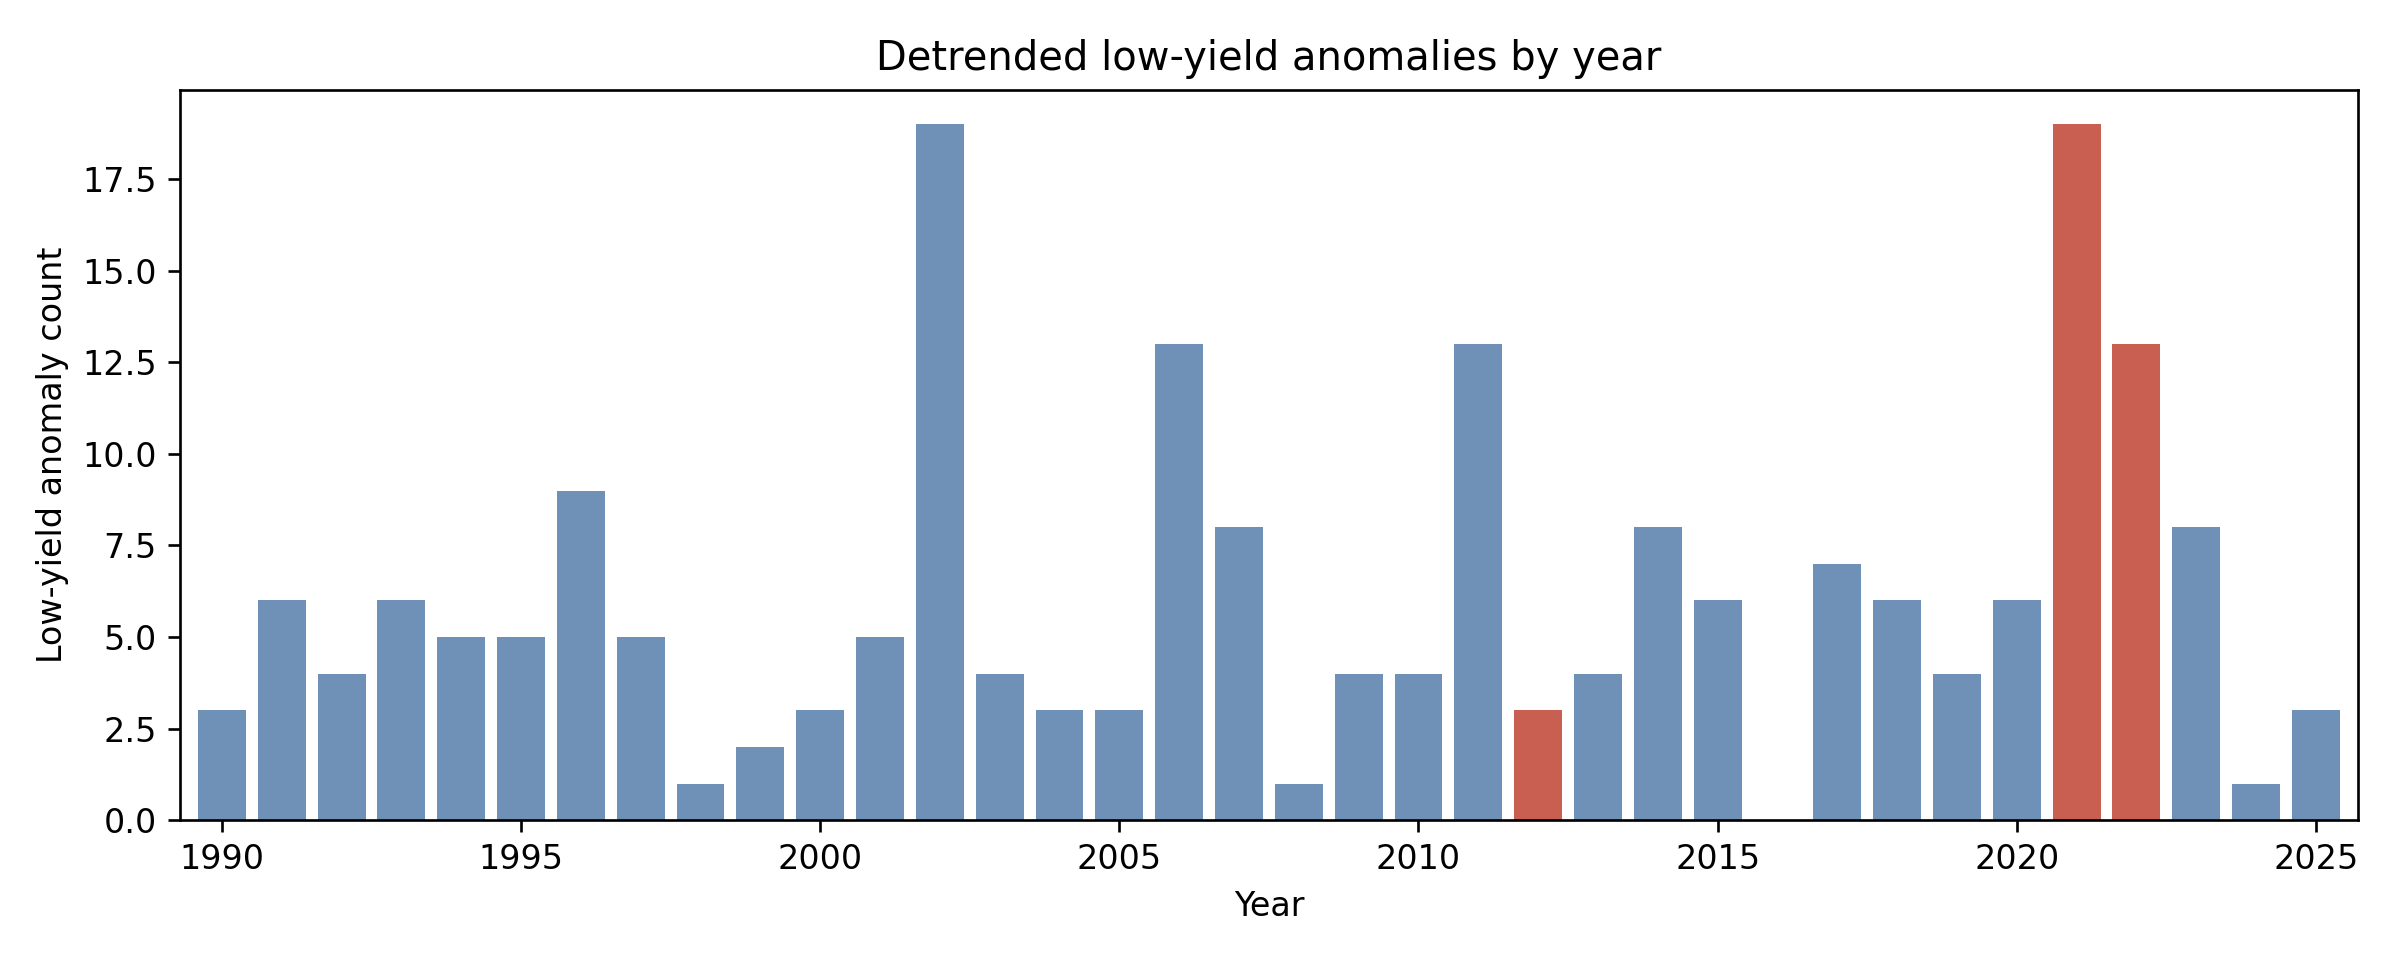
\includegraphics[width=0.86\linewidth]{fig02_anomaly_timeline.png}
  \caption{Detrended low-yield anomaly counts by year, with 2012, 2021, and 2022
  highlighted as plausibility-check years rather than training labels.}
  \label{fig:anomaly_timeline}
\end{figure}

Figure \ref{fig:anomaly_timeline} shows that the anomaly set is not evenly
distributed over time. The highlighted years are retained as sanity-check years
because broad heat and drought conditions were documented for 2012 and for parts of
the Northern Plains and western U.S. in 2021--2022
\citep{NOAA2012Drought,DroughtGov2021NorthernPlains,NOAA2022Drought}. Table
\ref{tab:model_performance} shows why the residual model is interpreted cautiously:
yield-level prediction is strong, but residual anomaly-magnitude prediction is weak,
so the XAI results are diagnostic explanations of fitted-model behavior.

\subsection{Feature and Driver Rankings}
Figure \ref{fig:shap_summary} indicates that the residual model relies on a mixture
of rainfall, dry-spell, heatwave, wetness, and cold-stress features rather than a
single variable family. This motivates grouping features by physical driver process
instead of interpreting isolated feature rankings alone.

\begin{figure}[!htbp]
  \centering
  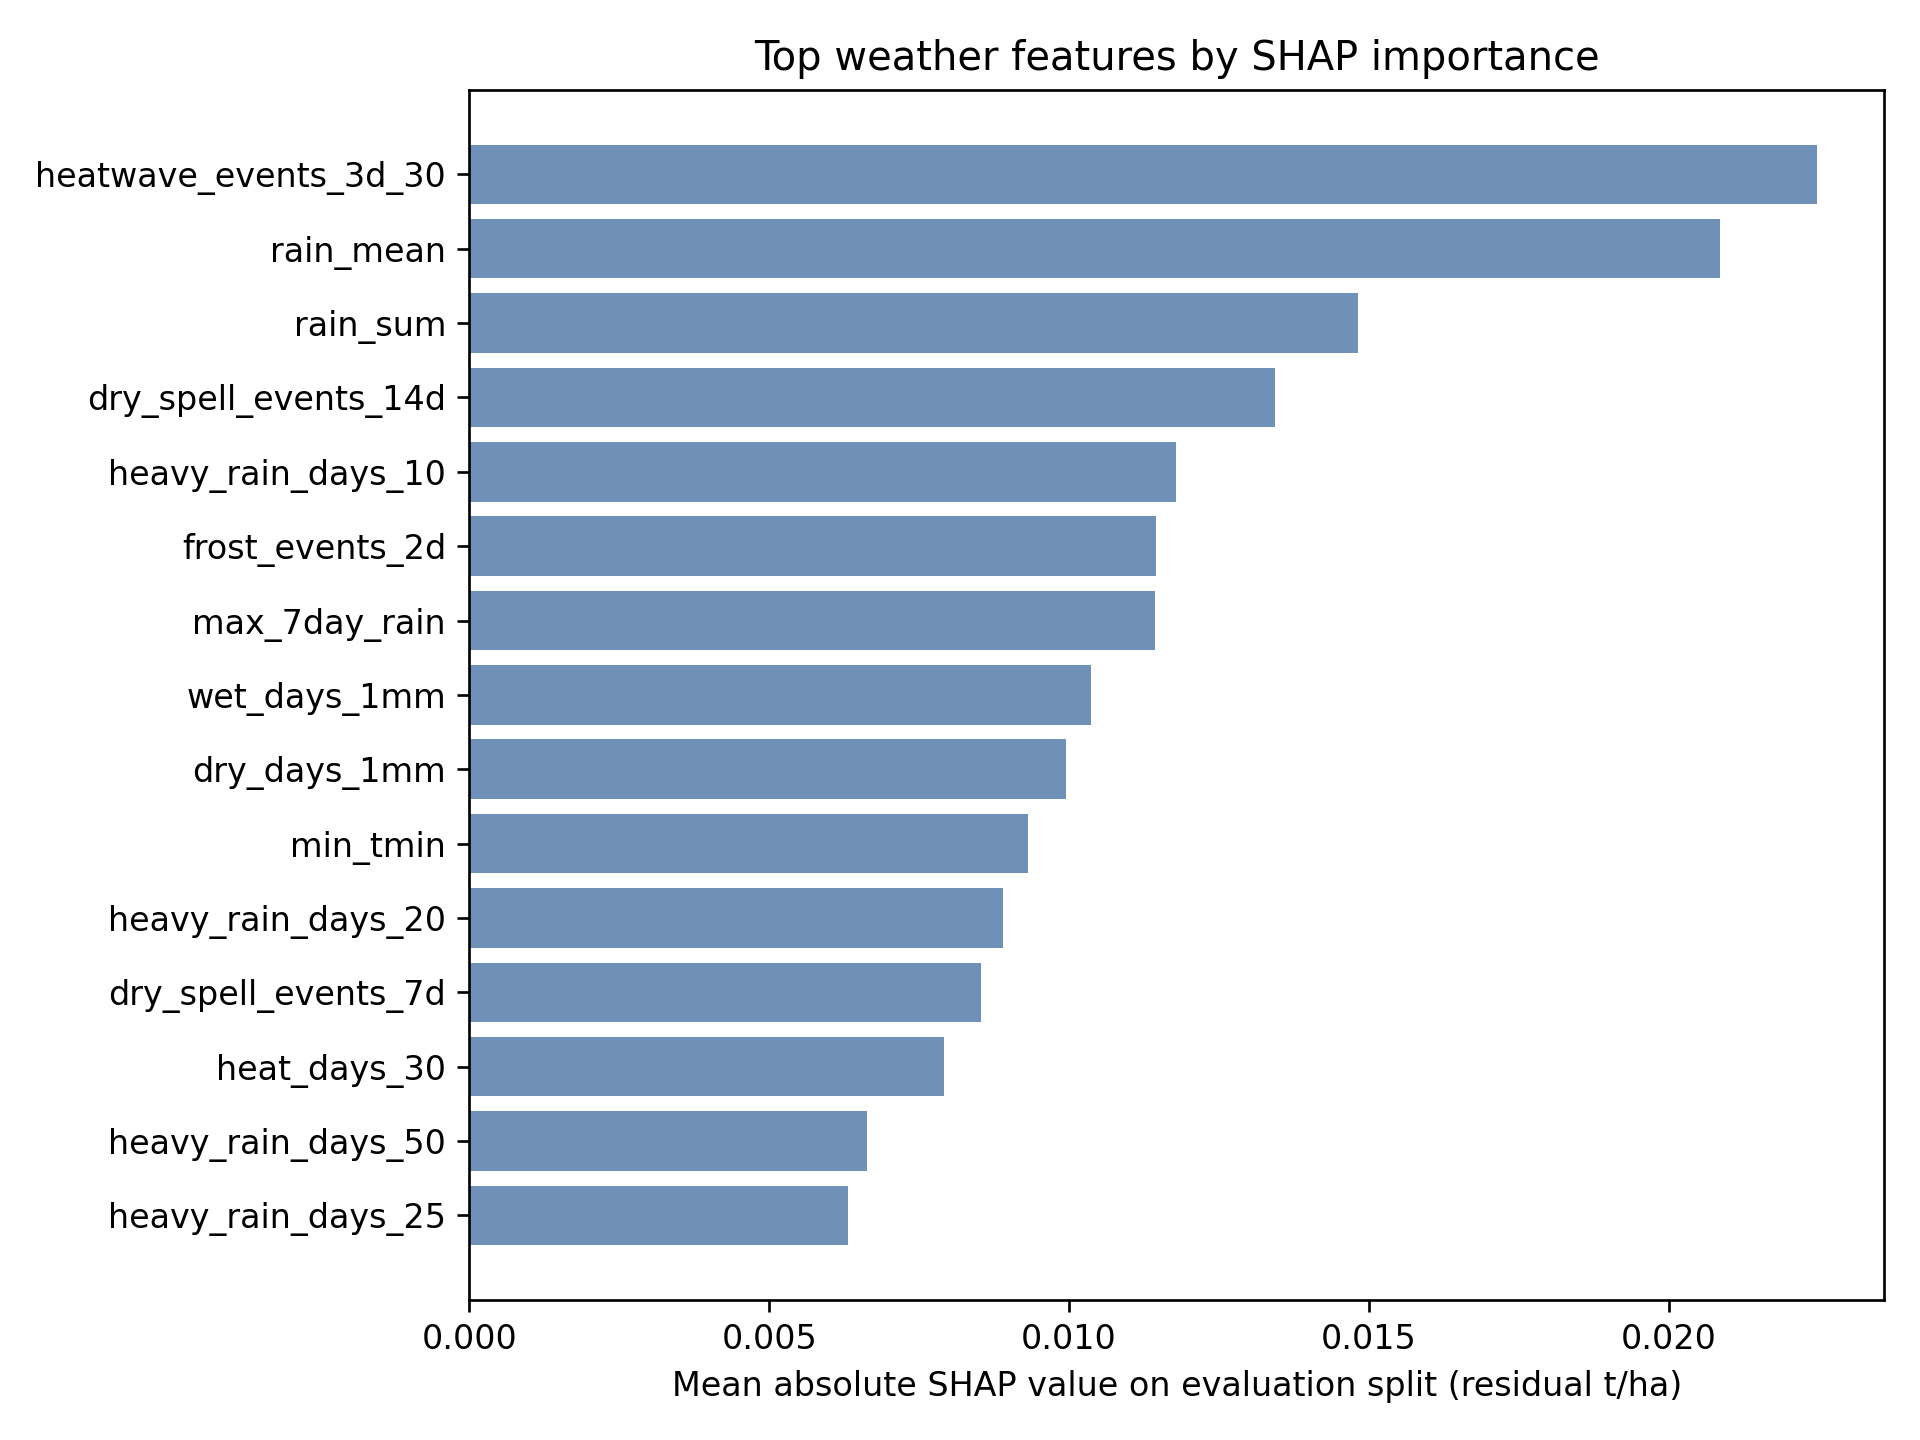
\includegraphics[width=0.82\linewidth]{fig03_shap_summary.png}
  \caption{Top weather features by mean absolute SHAP value in the residual model on
  the forward-time evaluation split.}
  \label{fig:shap_summary}
\end{figure}

Grouped SHAP shows a shift between forward-time evaluation rows and anomaly rows
(Figure \ref{fig:grouped_shap}). On the forward-time anomaly subset, heat and
drought are the two largest grouped contributions, with excess rain next. The
difference between evaluation-row and anomaly-only summaries is important: anomaly
explanation should not be reduced to global feature importance alone.

\begin{figure}[!htbp]
  \centering
  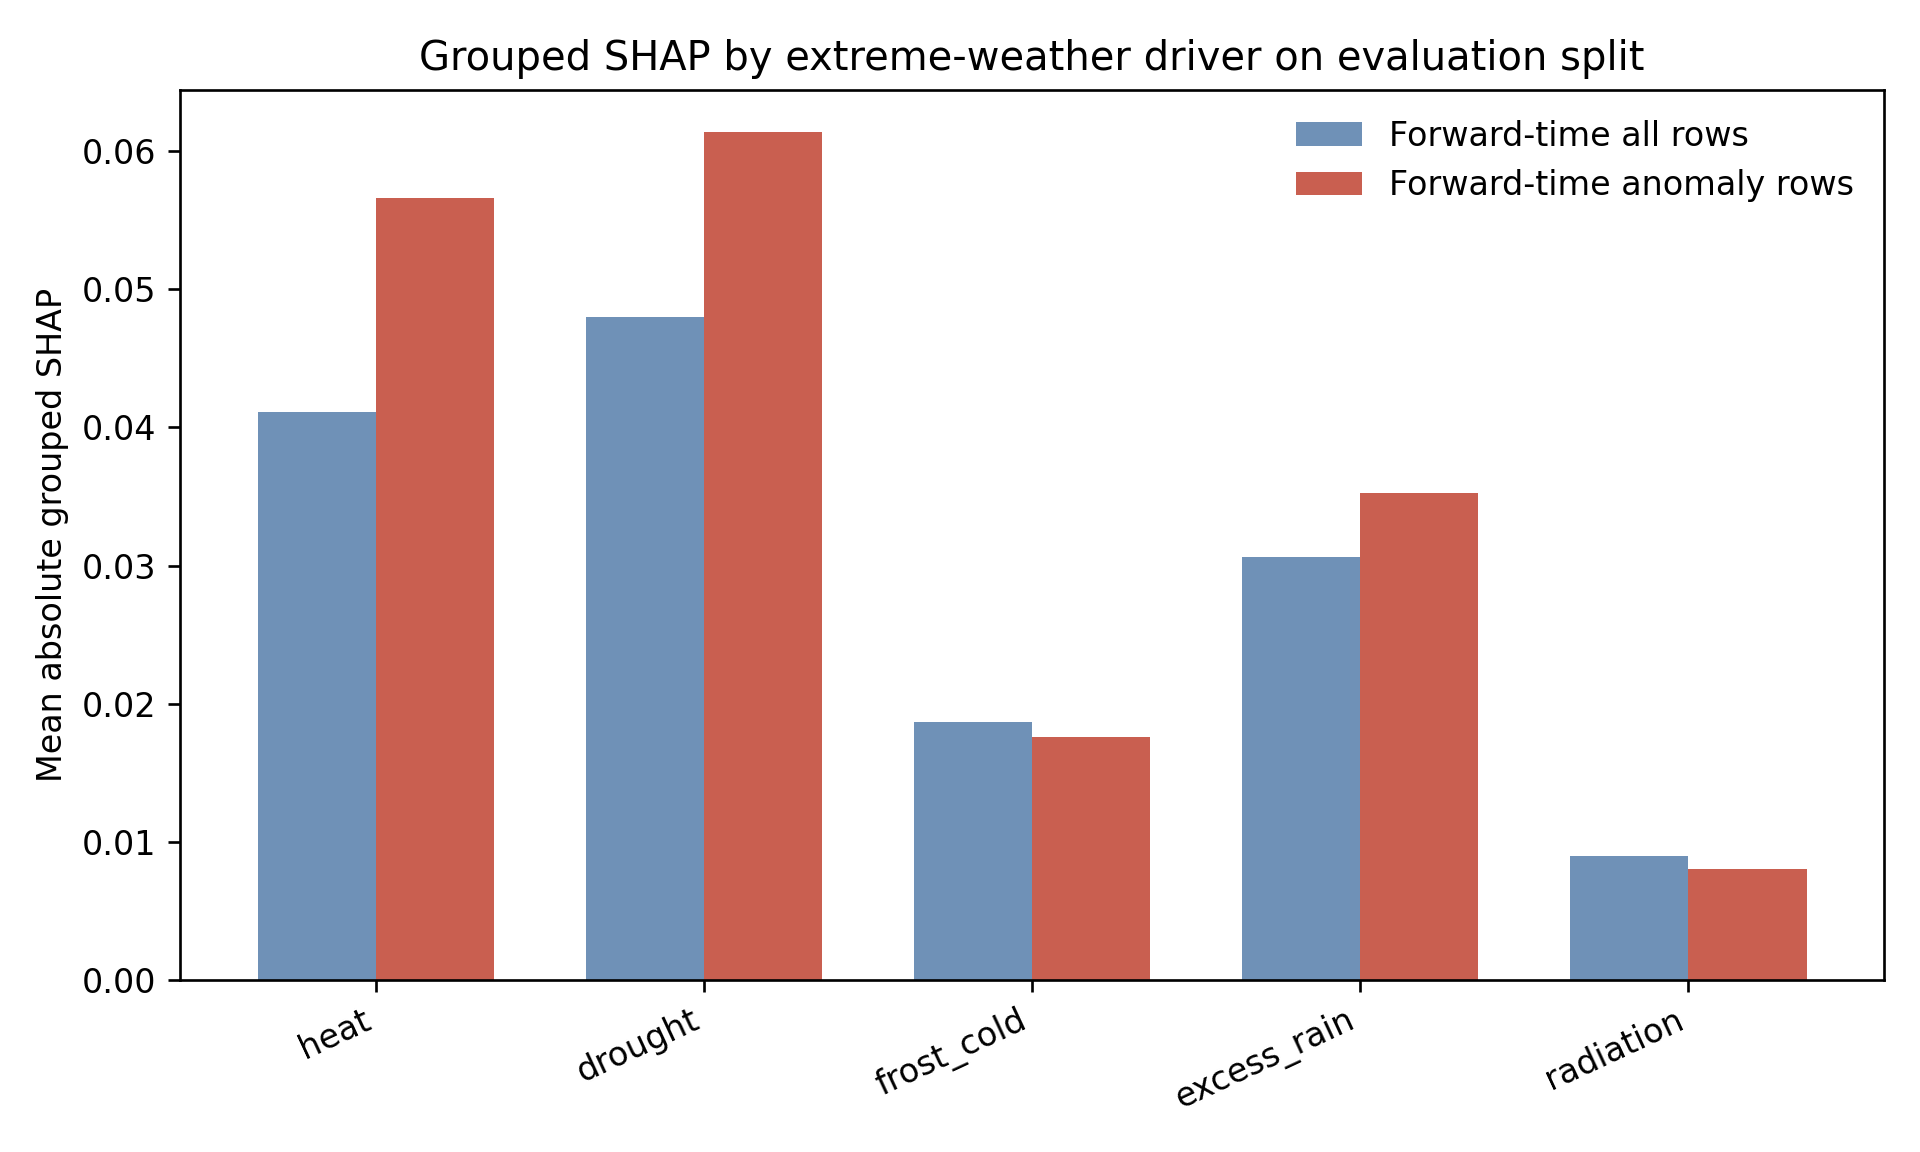
\includegraphics[width=0.82\linewidth]{fig04_grouped_shap.png}
  \caption{Grouped SHAP summaries for forward-time evaluation rows and anomaly rows.}
  \label{fig:grouped_shap}
\end{figure}

\input{tables/table05_driver_rankings.tex}

Table \ref{tab:driver_rankings} provides complementary global and anomaly-focused
views. Grouped SHAP, permutation, and ablation are all reported on the forward-time
evaluation split; LIME remains a selected-case check and is identified by its
smaller $n_{eval}$. Because the score units differ across methods, the table should
be read as a cross-method rank summary rather than an identical-scale statistical
comparison. Globally, heat is the strongest group under retraining ablation and
group permutation, while grouped SHAP ranks drought first. On anomaly rows, heat and
drought become co-leading signals: heat ranks first under group ablation and
selected LIME cases, while drought ranks first under grouped SHAP and group
permutation.

\begin{figure}[!htbp]
  \centering
  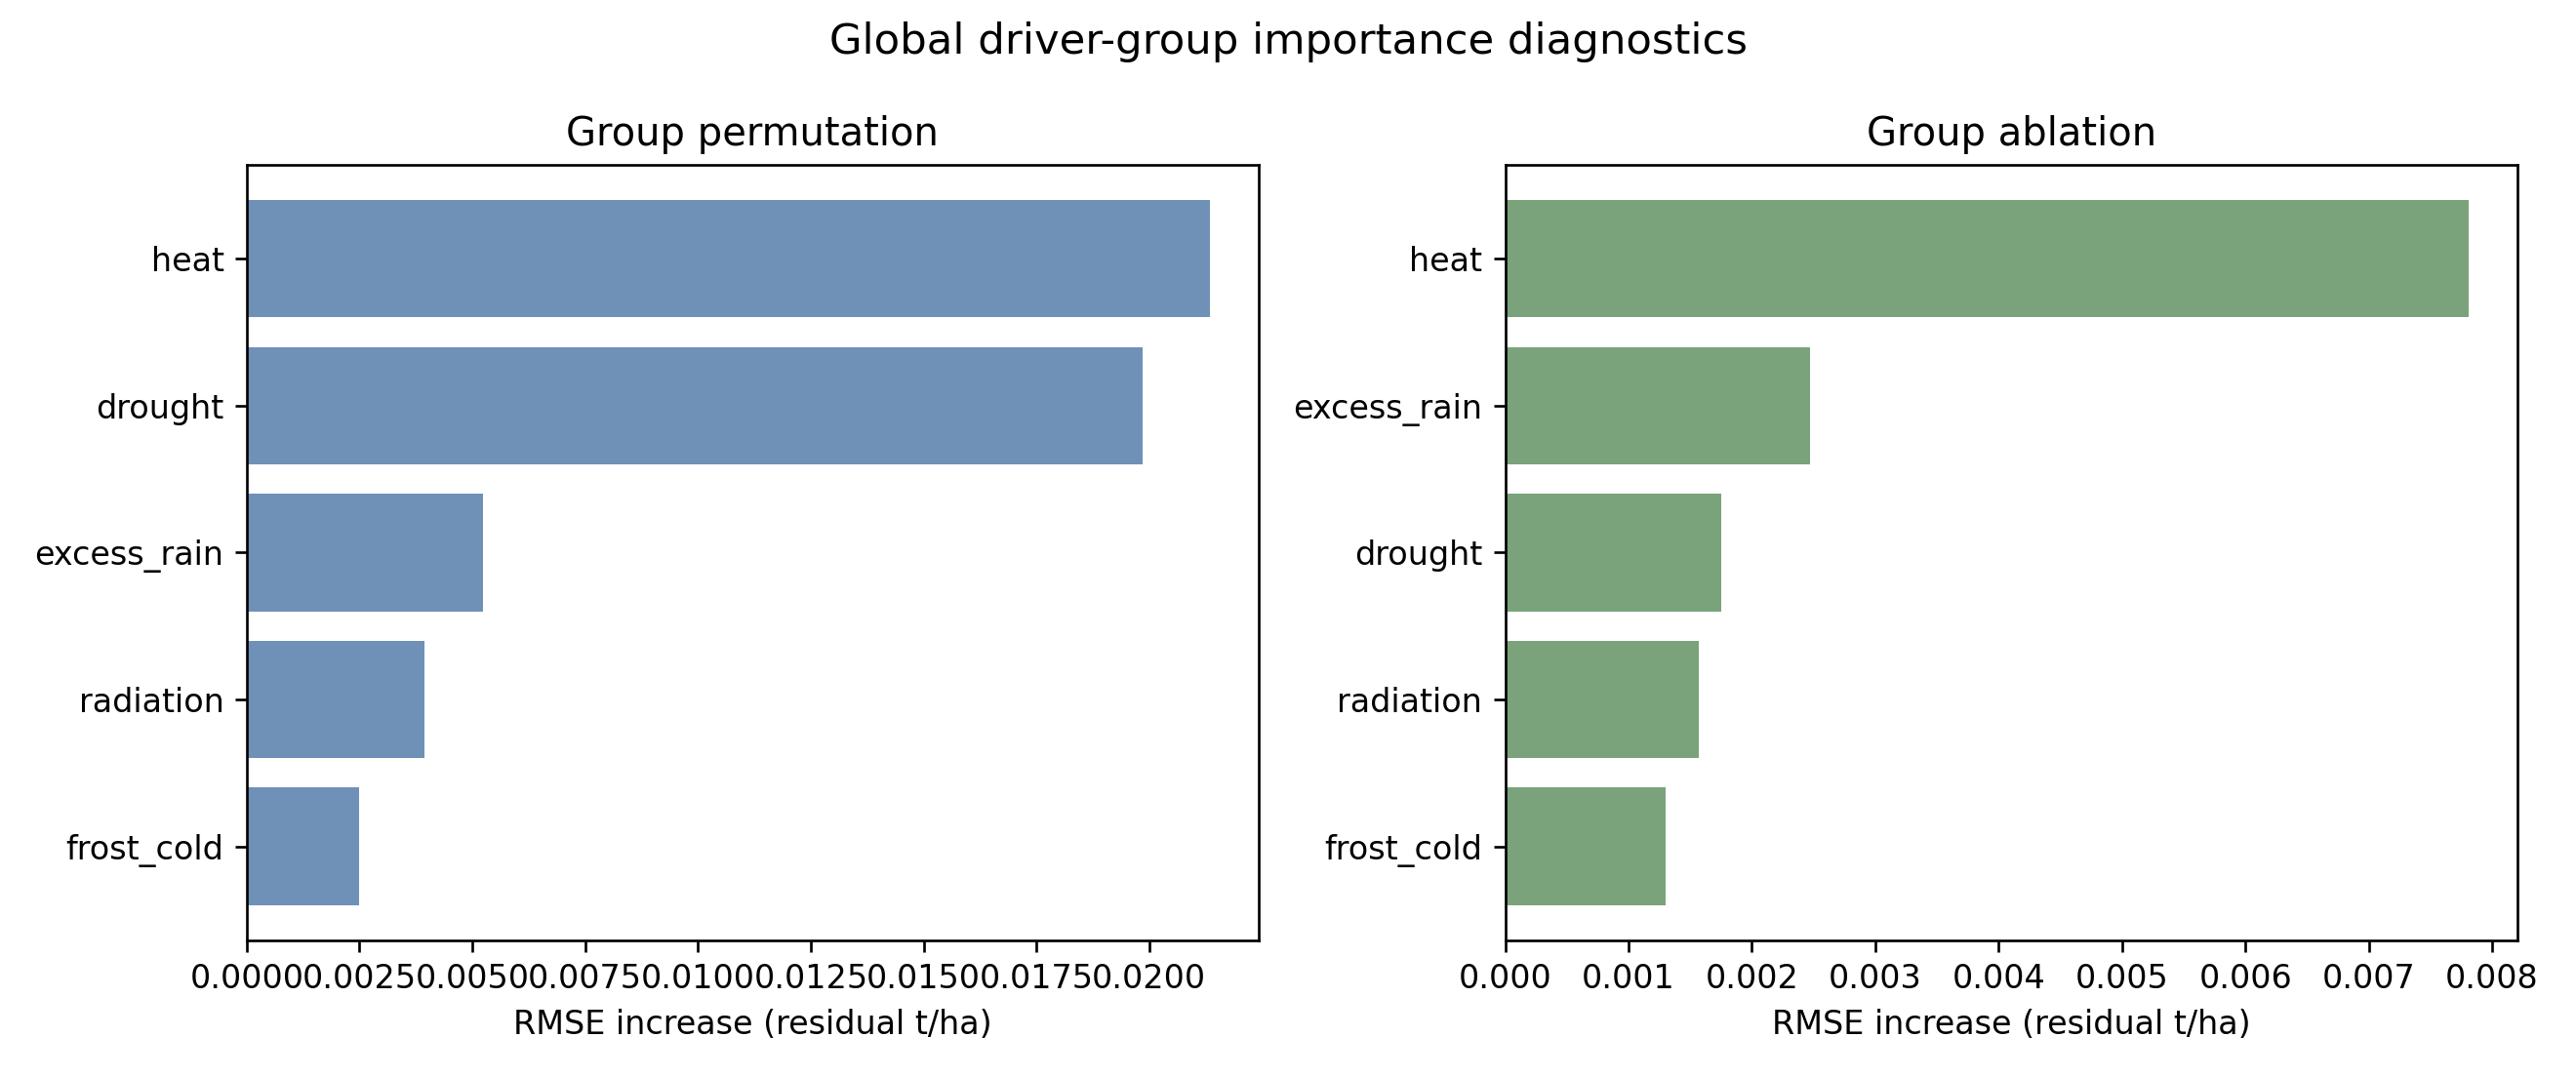
\includegraphics[width=0.9\linewidth]{fig05_group_importance.png}
  \caption{Global group permutation and group ablation importance measured by
  residual RMSE increase.}
  \label{fig:group_importance}
\end{figure}

Figure \ref{fig:group_importance} explains why method comparison is useful.
Permutation measures how much the fitted model depends on a driver group at
prediction time; ablation measures whether the model can compensate when the group is
removed and retrained. Heat ranks highest under both global diagnostics, suggesting
robust global reliance. Drought ranks strongly under permutation but less strongly
under retraining ablation, suggesting that drought information partly overlaps with
other rainfall and wetness features.

\subsection{Response Curves and Agreement}
ALE curves provide qualitative support for the driver rankings. Heat-related curves
generally decline at higher exposure levels, consistent with adverse
high-temperature behavior in the fitted residual model. Rainfall and dry-spell curves
are more nonlinear, suggesting that the model does not treat water stress as a simple
monotonic process.

\begin{figure}[!htbp]
  \centering
  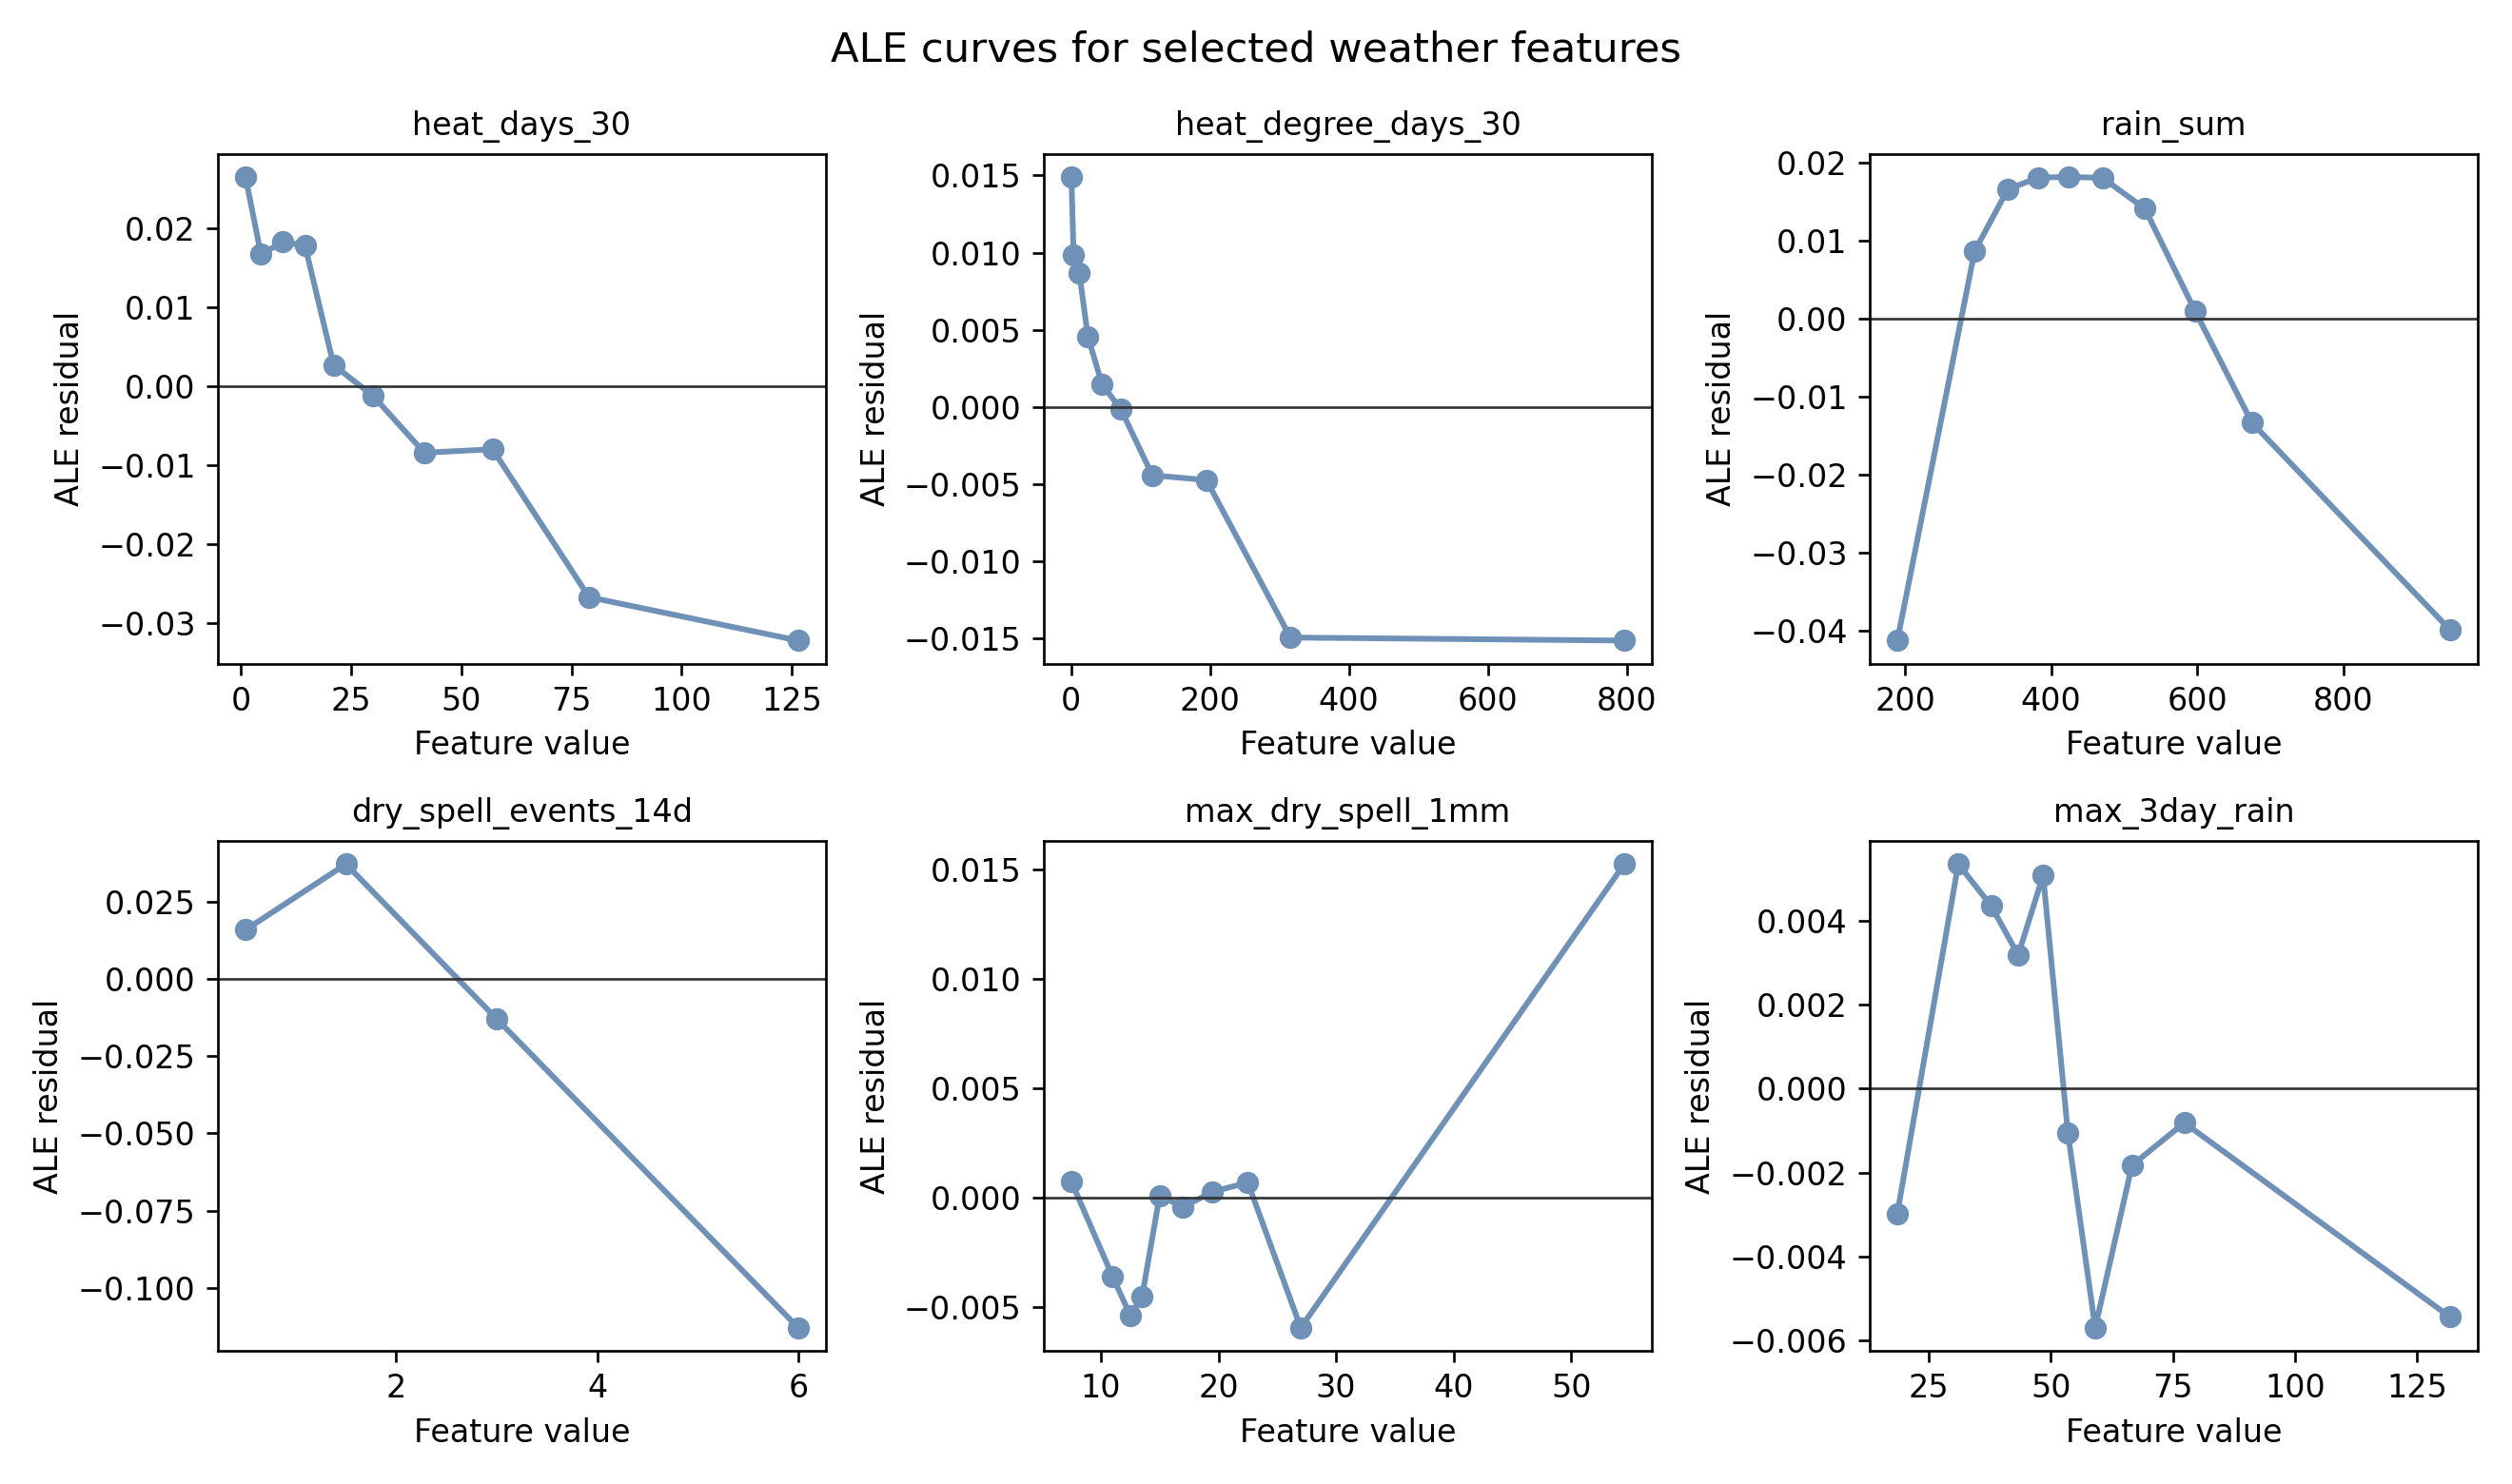
\includegraphics[width=0.95\linewidth]{fig07_ale_curves.png}
  \caption{ALE curves for selected heat, drought, and rainfall features.}
  \label{fig:ale}
\end{figure}

\begin{table}[!htbp]
\centering
\caption{Scale-free rank-one support summary across heterogeneous explanation methods.}
\label{tab:method_agreement}
\begingroup
\small
\setlength{\tabcolsep}{3pt}
\renewcommand{\arraystretch}{1.12}
\begin{tabularx}{\linewidth}{@{}>{\raggedright\arraybackslash}p{0.08\linewidth}>{\centering\arraybackslash}p{0.08\linewidth}>{\raggedright\arraybackslash}p{0.13\linewidth}>{\raggedright\arraybackslash}p{0.09\linewidth}>{\raggedright\arraybackslash}X>{\raggedright\arraybackslash}X@{}}
\toprule
scope & n methods & consensus driver & rank-1 votes & supporting methods & interpretation \\
\midrule
global & 3 & heat & 2/3 & group ablation, group permutation & Heat has majority support across global model-reliance diagnostics. \\
anomaly & 4 & drought; heat & 2/4 each & drought: group permutation, grouped SHAP; heat: group ablation, LIME selected cases & Heat and drought are co-leading anomaly-focused signals under rank-one support. \\
\bottomrule
\end{tabularx}
\endgroup
\end{table}


Table \ref{tab:method_agreement} summarizes rank-one support across heterogeneous
explanation methods. It should be read as a scale-free consensus summary, not as a
statistical test of driver importance. Figure \ref{fig:agreement} visualizes rank
positions rather than method-by-method rate estimates: darker/high-rank cells indicate
which driver groups are placed near the top by each method. Global diagnostics give
majority rank-one support to heat, while anomaly-focused explanations split their
rank-one support between heat and drought.

\begin{figure}[!htbp]
  \centering
  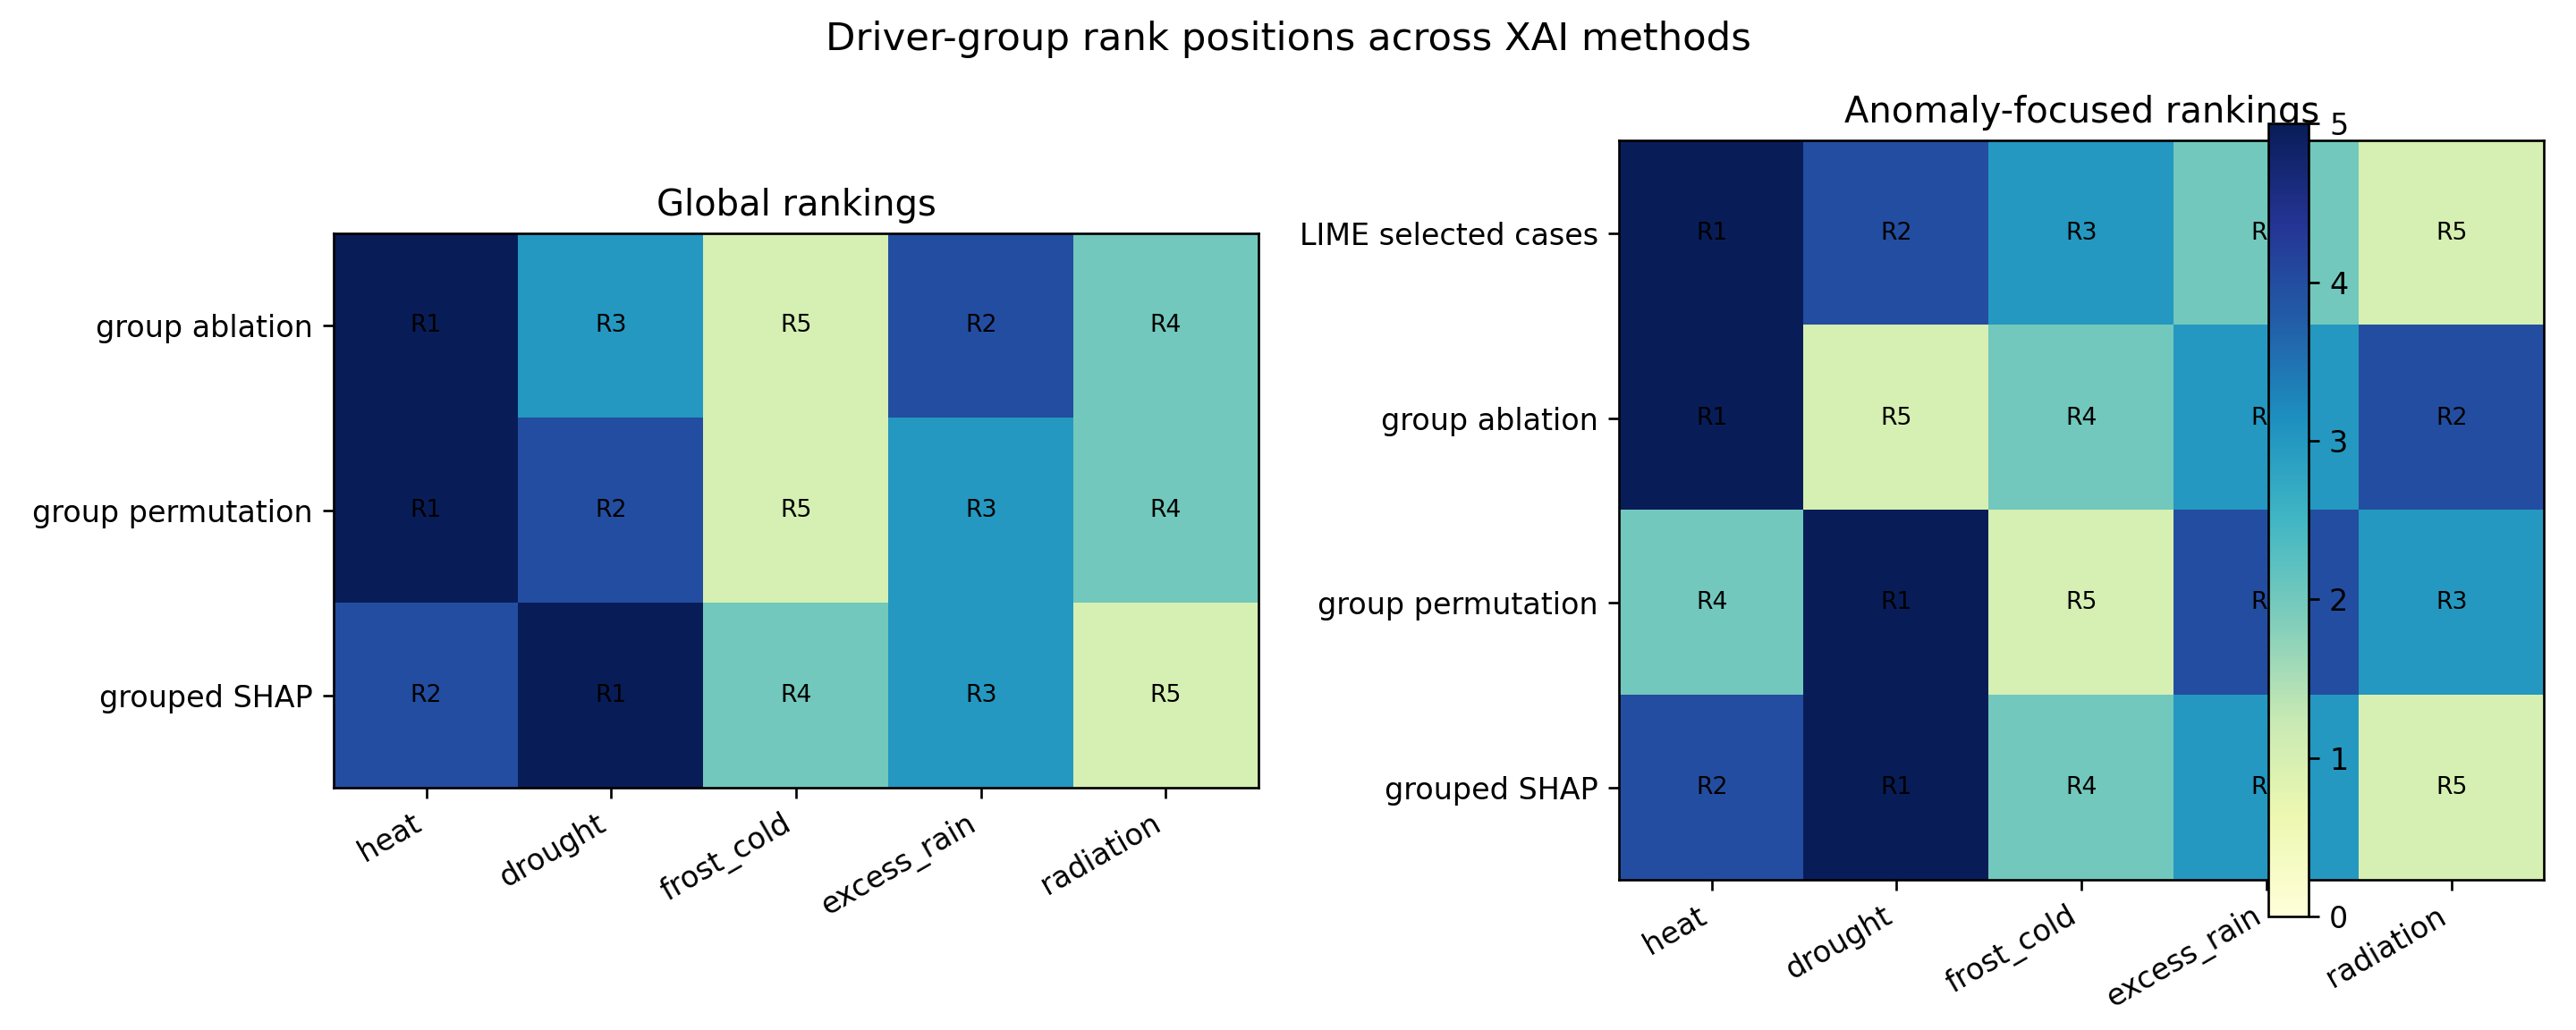
\includegraphics[width=0.92\linewidth]{fig08_method_agreement.png}
  \caption{Driver-group rank positions across global and anomaly-focused XAI methods.}
  \label{fig:agreement}
\end{figure}

\begin{table}[!htbp]
\centering
\caption{Six selected event-level method-sensitivity checks using grouped SHAP and LIME.}
\label{tab:event_explanations}
\resizebox{\linewidth}{!}{%
\begin{tabular}{@{}lllllll@{}}
\toprule
crop & state & year & trend\_residual\_z & grouped\_shap\_driver & lime\_driver & drivers\_agree \\
\midrule
Canola & North Dakota & 2012 & -1.49 & heat & heat & yes \\
Oats & Kansas & 2012 & -2.33 & heat & drought & no \\
Barley & South Dakota & 2021 & -2.98 & heat & heat & yes \\
Wheat & Washington & 2021 & -2.92 & heat & heat & yes \\
Oats & Oklahoma & 2022 & -3.44 & drought & heat & no \\
Wheat & Nebraska & 2022 & -2.64 & drought & drought & yes \\
\bottomrule
\end{tabular}
}
\end{table}


Table \ref{tab:event_explanations} reports six representative cases from the
selected LIME case-study set and illustrates selected case-level method
sensitivity. Its purpose is not to validate event-level correctness. Agreement
between grouped SHAP and LIME in four of six selected cases provides stronger
diagnostic support for those examples, while the two disagreements indicate that
event-level driver assignments should be treated cautiously and not reported as
robust single-driver claims.

\section{Discussion}
The multi-method comparison supports a more nuanced conclusion than a single ranking
would provide. Heat is the strongest global model-reliance driver: both group
permutation and retraining ablation place heat first in the forward-time evaluation
setting. Anomaly-focused explanations are more method-sensitive. Drought ranks first
in evaluation-scope grouped SHAP and anomaly-row permutation, while heat ranks first
in anomaly-row ablation and selected LIME cases. Excess rain is a meaningful
secondary signal because rainfall and wetness features appear in feature-level and
grouped summaries.

Method disagreement is informative. SHAP describes additive contributions within the
fitted tree model; permutation measures prediction-time dependence; retraining
ablation measures whether other variables can substitute for a removed group; ALE
describes response shape; and LIME provides selected local surrogate checks. Weather
features are correlated, so methods that answer different questions should not agree
perfectly. The agreement protocol clarifies which driver claims are stable across
several lenses and which are method-sensitive.

Several limitations remain. The dataset is state-level and uses representative
coordinates, so it cannot capture within-state weather, soil, irrigation, cultivar,
or management heterogeneity. Detrending choices influence which rows are labelled as
anomalies. The residual model has limited skill for anomaly magnitudes, which narrows
the claim to diagnostic explanation of fitted-model behavior. Finally, the analysis
is not a formal climate-event attribution study; that task requires a different
causal and probabilistic framework \citep{Otto2017,Oldenborgh2021,Otto2023}.

\section{Conclusion}
This study presents a reproducible multi-method XAI protocol for explaining
detrended crop-yield anomalies. By combining anomaly screening, residual modeling,
SHAP, grouped SHAP, group permutation, group ablation, ALE, selected LIME cases, and
method agreement, the analysis avoids relying on a single explanation method. The
main empirical pattern is that heat is the strongest global model-reliance driver,
while heat and drought are co-leading anomaly-focused signals depending on the
explanation method. The approach provides a cautious, transparent bridge between
crop-yield prediction and diagnostic
interpretation.

\bibliographystyle{plainnat}
\bibliography{references}
\end{document}
